\documentclass[12pt]{article}
\usepackage[a4paper, margin=2.5cm]{geometry}
\usepackage{xeCJK} % 中文支持
\usepackage{amsmath, amssymb}
\usepackage{graphicx}
\usepackage{caption}
\usepackage{subcaption}
\usepackage{hyperref}
\usepackage{natbib}
\usepackage{fancyhdr}
\usepackage{titlesec}
\usepackage{physics}
\usepackage{listings}
\usepackage{ctex}
\usepackage{xcolor}
\usepackage[most]{tcolorbox}
% 用来设置附录中代码的样式

\lstset{
    basicstyle          =   \sffamily,          % 基本代码风格
    keywordstyle        =   \bfseries,          % 关键字风格
    commentstyle        =   \rmfamily\itshape,  % 注释的风格,斜体
    stringstyle         =   \ttfamily,  % 字符串风格
    flexiblecolumns,                % 别问为什么,加上这个
    numbers             =   left,   % 行号的位置在左边
    showspaces          =   false,  % 是否显示空格,显示了有点乱,所以不现实了
    numberstyle         =   \zihao{-5}\ttfamily,    % 行号的样式,小五号,tt等宽字体
    showstringspaces    =   false,
    captionpos          =   t,      % 这段代码的名字所呈现的位置,t指的是top上面
    frame               =   lrtb,   % 显示边框
}
\lstdefinestyle{verilog-style}{
    language=Verilog,
    basicstyle=\ttfamily\small,
    keywordstyle=\color{blue},
    commentstyle=\color{gray},
    stringstyle=\color{orange},
    numbers=none,
    %numberstyle=\tiny,
    %stepnumber=1,
    %numbersep=5pt,
    showstringspaces=false,
    breaklines=true,
    frame=single
}
\lstdefinestyle{Python}{
    language        =   Python, % 语言选Python
    basicstyle      =   \zihao{-5}\ttfamily,
    numberstyle     =   \zihao{-5}\ttfamily,
    keywordstyle    =   \color{blue},
    keywordstyle    =   [2] \color{teal},
    stringstyle     =   \color{magenta},
    commentstyle    =   \color{red}\ttfamily,
    breaklines      =   true,   % 自动换行,建议不要写太长的行
    columns         =   fixed,  % 如果不加这一句,字间距就不固定,很丑,必须加
    basewidth       =   0.5em,
}
% 字体设置(可根据系统修改)
\setCJKmainfont{SimSun} % 宋体
\setmainfont{Times New Roman}

% 调整页眉高度,避免 fancyhdr 警告
\setlength{\headheight}{14.5pt} 

% 页眉设置
\pagestyle{fancy}
\fancyhf{}
\fancyhead[L]{VLA}
\fancyhead[R]{\thepage}

% 标题格式
\titleformat{\section}{\large\bfseries}{\thesection.}{0.5em}{}
\titleformat{\subsection}{\normalsize\bfseries}{\thesubsection.}{0.5em}{}

% 封面信息
\title{Vision-Language-Action \\ \large 一些研究笔记}
\author{ghx \quad \\}
\date{\today}

\begin{document}

\maketitle

\begin{abstract}
大一在fhh老师实验室学习的笔记、看文献的总结(我会什么? )
\end{abstract}

\section{机器人大脑VLA的发展史\cite{vla_history_csdn}}

\subsection{目前VLM(Vision-Language modle)赋能机器人的两条路线}
一是直接提示VLM规划的更细:VLM负责理解任务和环境,加约束提升动作合理性,让 VLM 充当“高层指路人” (planner) ,再用低层执行器完成具体动作,尤其加入逻辑约束、语言结构来增强泛化与可控性,代表文章\cite{vlm_constrained_planning}。 (来自chatGTP)

二是从Robotics VLM到VLA,包含RT2、OpenVLA、π0等代表性的VLA模型。在 VLM 上加入动作专家,直接输出 end-to-end 行为(端到端) ,将 VLM 本身“再训练”或“微调”,使其不仅能理解图文语言,还能直接控制机器人动作(来自chatGTP) 。
其中代表文章是\cite{vla_history_csdn}。即我们所称的VLA,感觉这一方向应当是主流方向

\subsection{之前的VLA相关工作}

\subsubsection{微调}
早期的研究者Jang等人(2022)和Lynch\&Sermanet(2020)等早期研究已经训练了一个Vision Encoder和一个Language Encoder,来学习操纵任务中输入语言和视觉数据的表示。
但最近的一些工作则直接采用预训练模型(提前在大量通用数据上训练好的 AI 模型,具备“通用能力”,可以迁移到其他任务中继续使用或微调)来获取优质表示,并从头开始训练策略模型或微调整个模型

\begin{figure}[ht]  % 推荐用 [ht] 比 [h] 更稳定
\centering
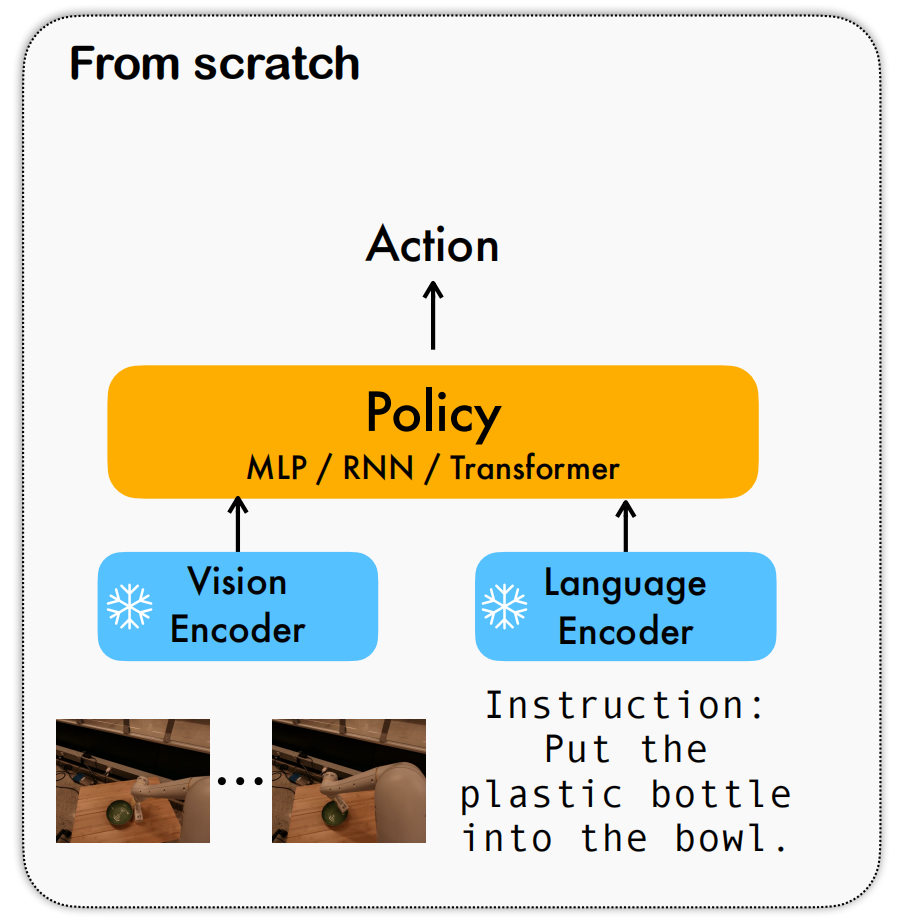
\includegraphics[width=0.6\textwidth]{pic1.png}
\caption{微调}
\end{figure}

\subsubsection{LLM规划}
一些方法已经利用大型语言模型(LLMs)作为强大的零样本计划器,例如SayCan Ahn等人(2022),以生成预定义的分步计划,并在给定任务上提供人工交互提示,随后指示不同的预训练低级策略来执行这些计划并完成多个任务
有些方法会把LLM当作计划器使用,以为LLM已经具备了“常识推理和任务拆解的能力” ,它可以在没有见过这个具体任务的训练样本的情况下,生成合理的执行步骤。

LLM会将一个复杂任务分为几个步骤,在这个过程中人类可以通过语言提示来微调或引导计划的方向,然后分发给实现训练好的低级控制器(low-level policies)去完成,这些低级策略就像机器人的“技能库” ,是事先训练好的动作执行模块。这种方法可以支持机器人执行多个复杂任务,并具备泛化能力。
\begin{figure}[ht]  % 推荐用 [ht] 比 [h] 更稳定
\centering
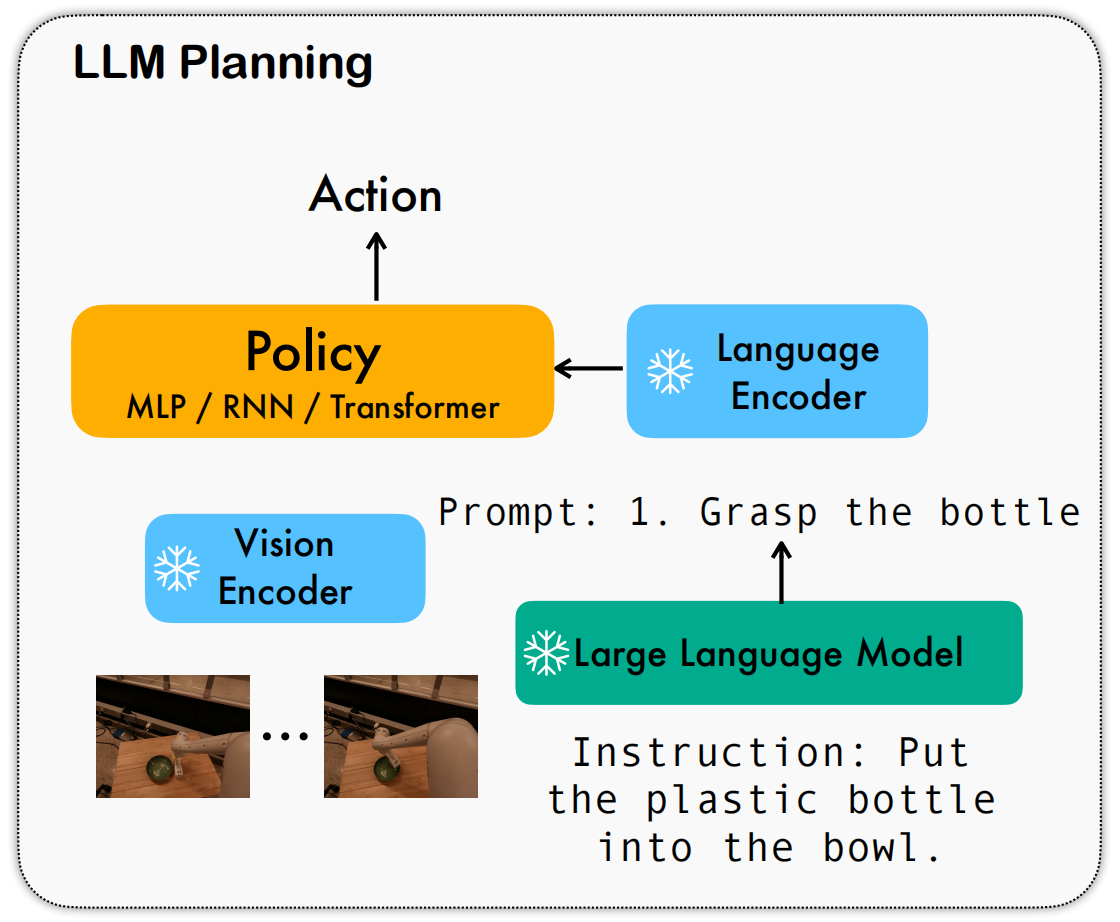
\includegraphics[width=0.6\textwidth]{pic2.png}
\caption{LLM规划}
\end{figure}

\subsubsection{协同精调Co-Fine-Tuning}
Dries等人提出了540B PaLM-E模型,展示了一种不同的利用预训练视觉和语言模型的方法。

\begin{tcolorbox}[colback=blue!5!white, colframe=blue!75!black, title=以下内容来自ChatGTP]
Dries 等人提出的 PaLM-E 模型是怎么做的?

PaLM-E 是 Google 在 2023 年提出的一个超大型机器人多模态模型(参数量高达 5400 亿),具体做法包括:
\\1. 使用多个预训练模型提取视觉信息:
他们用一些已经训练好的视觉模型(比如 ViT)来处理场景图像,并把这些图像信息传给 PaLM 模型。
\\2. 使用 PaLM(大语言模型)作为核心主干:PaLM 是一个超大的语言模型,原本是为自然语言处理设计的,现在它作为整个系统的“思考中枢”。
\\3. 使用来自多个来源的视觉+语言训练数据,比如:

\hspace*{2em}移动操作任务的问答数据(“怎么打开冰箱?”) 

\hspace*{2em}图像描述任务(Image Captioning)

\hspace*{2em}视觉问答任务(Visual Question Answering)

这些数据帮助模型理解“看到的画面 + 听到的指令”之间的联系
\\4.端到端地精调整个模型(协同精调)
整个 VLM(视觉语言模型)是一起训练的,不是分开训练后拼起来的,
这就保证了视觉、语言、动作之间的联系是协调一致地学出来的。
\\5. 类似LLM规划,也需要低级动作策略
即使模型能输出“多步计划”,真正去抓、放、推这些动作,还是需要训练好的低层策略(技能库)去执行。
\end{tcolorbox}

这是一种 把视觉模型 + 语言模型作为整体一起端到端训练(fine-tune) 的方法。
不像之前那样把视觉部分、语言部分、控制部分分开训练,而是 “联合优化整套系统” ,具体而言,如下三点:

1.通过使用移动操作问答数据以及从Web收集的图像标题和视觉问答数据等辅助视觉语言训练数据

2.通过使用移动操作问答数据以及从Web收集的图像标题和视觉问答数据等辅助视觉语言训练数据

3.他们通过端到端协同微调整个VLM来训练模型生成由语言描述的预定义多步计划,与SayCan类似,他们需要低级控制策略来执行生成的计划

\begin{figure}[ht]  % 推荐用 [ht] 比 [h] 更稳定
\centering
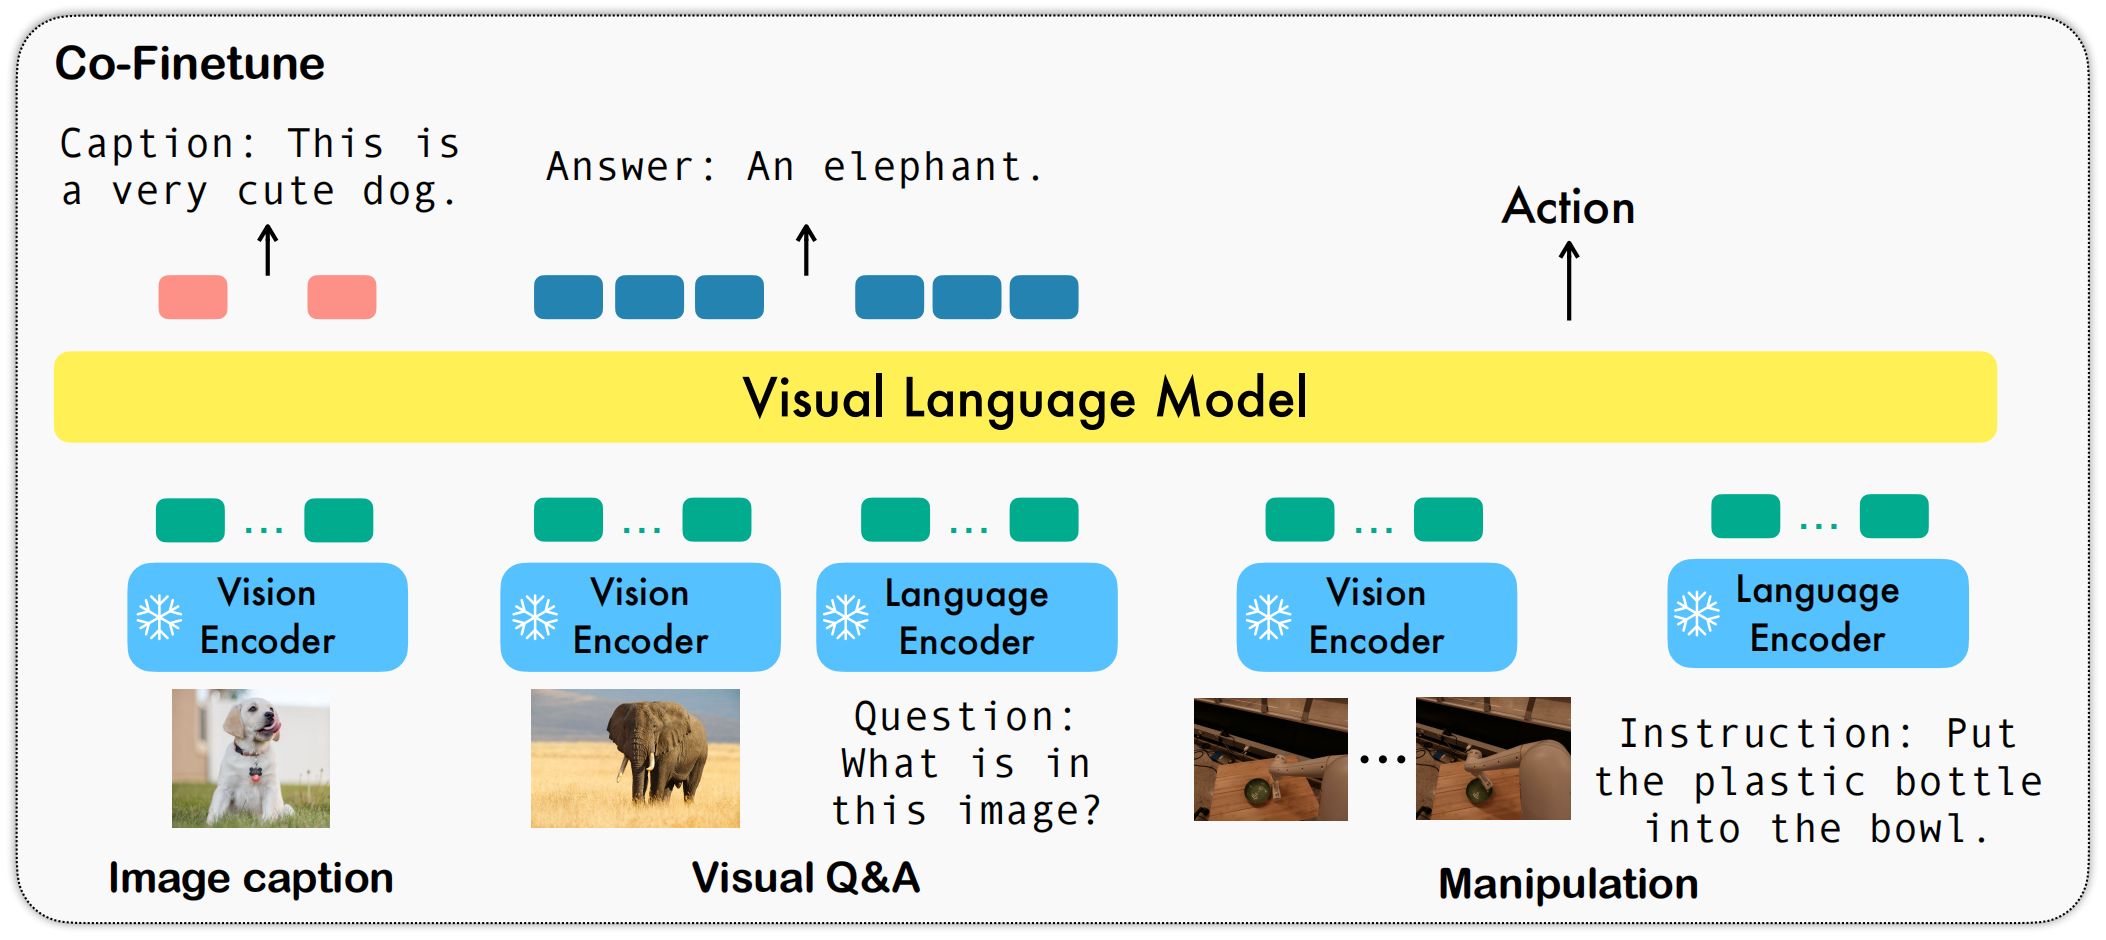
\includegraphics[width=0.9\textwidth]{pic3.png}
\caption{CFT}
\end{figure}
然而,他们的方法揭示了VLMs在适应机器人操作方面具有潜力,但是他们关键性的协同微调训练策略需要大量规模化Web数据、视觉语言数据和低级机器人动作。此外,VLMs及其所使用的数据是私有化的,这使得每位机器人从业者难以实施这样的解决方案

\subsubsection{总结}
尽管之前的模型在一定程度上弥合了机器人操作任务中视觉和语言之间的差距,但它们要么专注于低级技能策略(如SayCan和PaLM-E),要么训练一个庞大的整体模型(如RT-1),或者需要大量视觉语言数据和计算资源来确保学习操作策略时不会忽视视觉与语言之间重要的对齐关系

相比这些工作,RoboFlamingo是一个简单而直观的解决方案,可以轻松适应现有VLM(本文使用OpenFlamingo)并只需微调少量操作演示

\subsection{RoboFlamingo: Vision Encoder + Feature Fusion Decoder + Policy Head}
具体而言,RoboFlamingo利用已有的基于图像 - 文本对的视觉语言基础模型,通过训练端到端的方式生成机器人每一步的 relative action。
模型的主要模块包含了 vision encoder,feature fusion decoder 和 policy head 三个模块

以下是这三个模块分别要做的事:

1.Vision encoder 模块先将当前视觉观测输入到 ViT (一种新型图像识别模型,把图像当作“句子”来处理,用 NLP(自然语言处理)领域的 Transformer 架构来处理视觉任务,而非卷积)中,并通过 resampler 对 ViT 输出的 token 进行 down sample

2.Feature fusion decoder 将 text token 作为query,并在每个 layer 中先将 vision encoder 的 output 作为 key和value 进行 cross attention

注意,在交叉注意力中,什么做Q,什么做K V确实容易混淆,有的新闻稿便会弄错,怎么防止搞错呢?
i)  可以简单粗暴的把Q定义为主人,K V定义为客人,主人一般邀请客人到家交流,而在我们面对Feature fusion decoder时,它里面的text token当然就是主人,故自然作为query,然后把vision encoder 的 output 拿过来做cross attention,而拿过来的output自然便作为客人邀请过来了,故而是key和value
ii) 其实包括transformer中decoder的第二个注意力层便也有类似之意

3.最后,对 feature fusion decoder 进行 max pooling 后将其送入 policy head 中
policy head 根据 feature fusion decoder 输出的当前和历史 token 序列直接输出当前的 7 DoF relative action(包括6-dim 的机械臂末端位姿和 1-dim 的 gripper open/close)

在训练过程中,RoboFlamingo 利用预训练的 ViT、LLM 和 Cross Attention 参数,并只微调 resampler、cross attention 和 policy head 的参数

\begin{figure}[ht]  % 推荐用 [ht] 比 [h] 更稳定
\centering
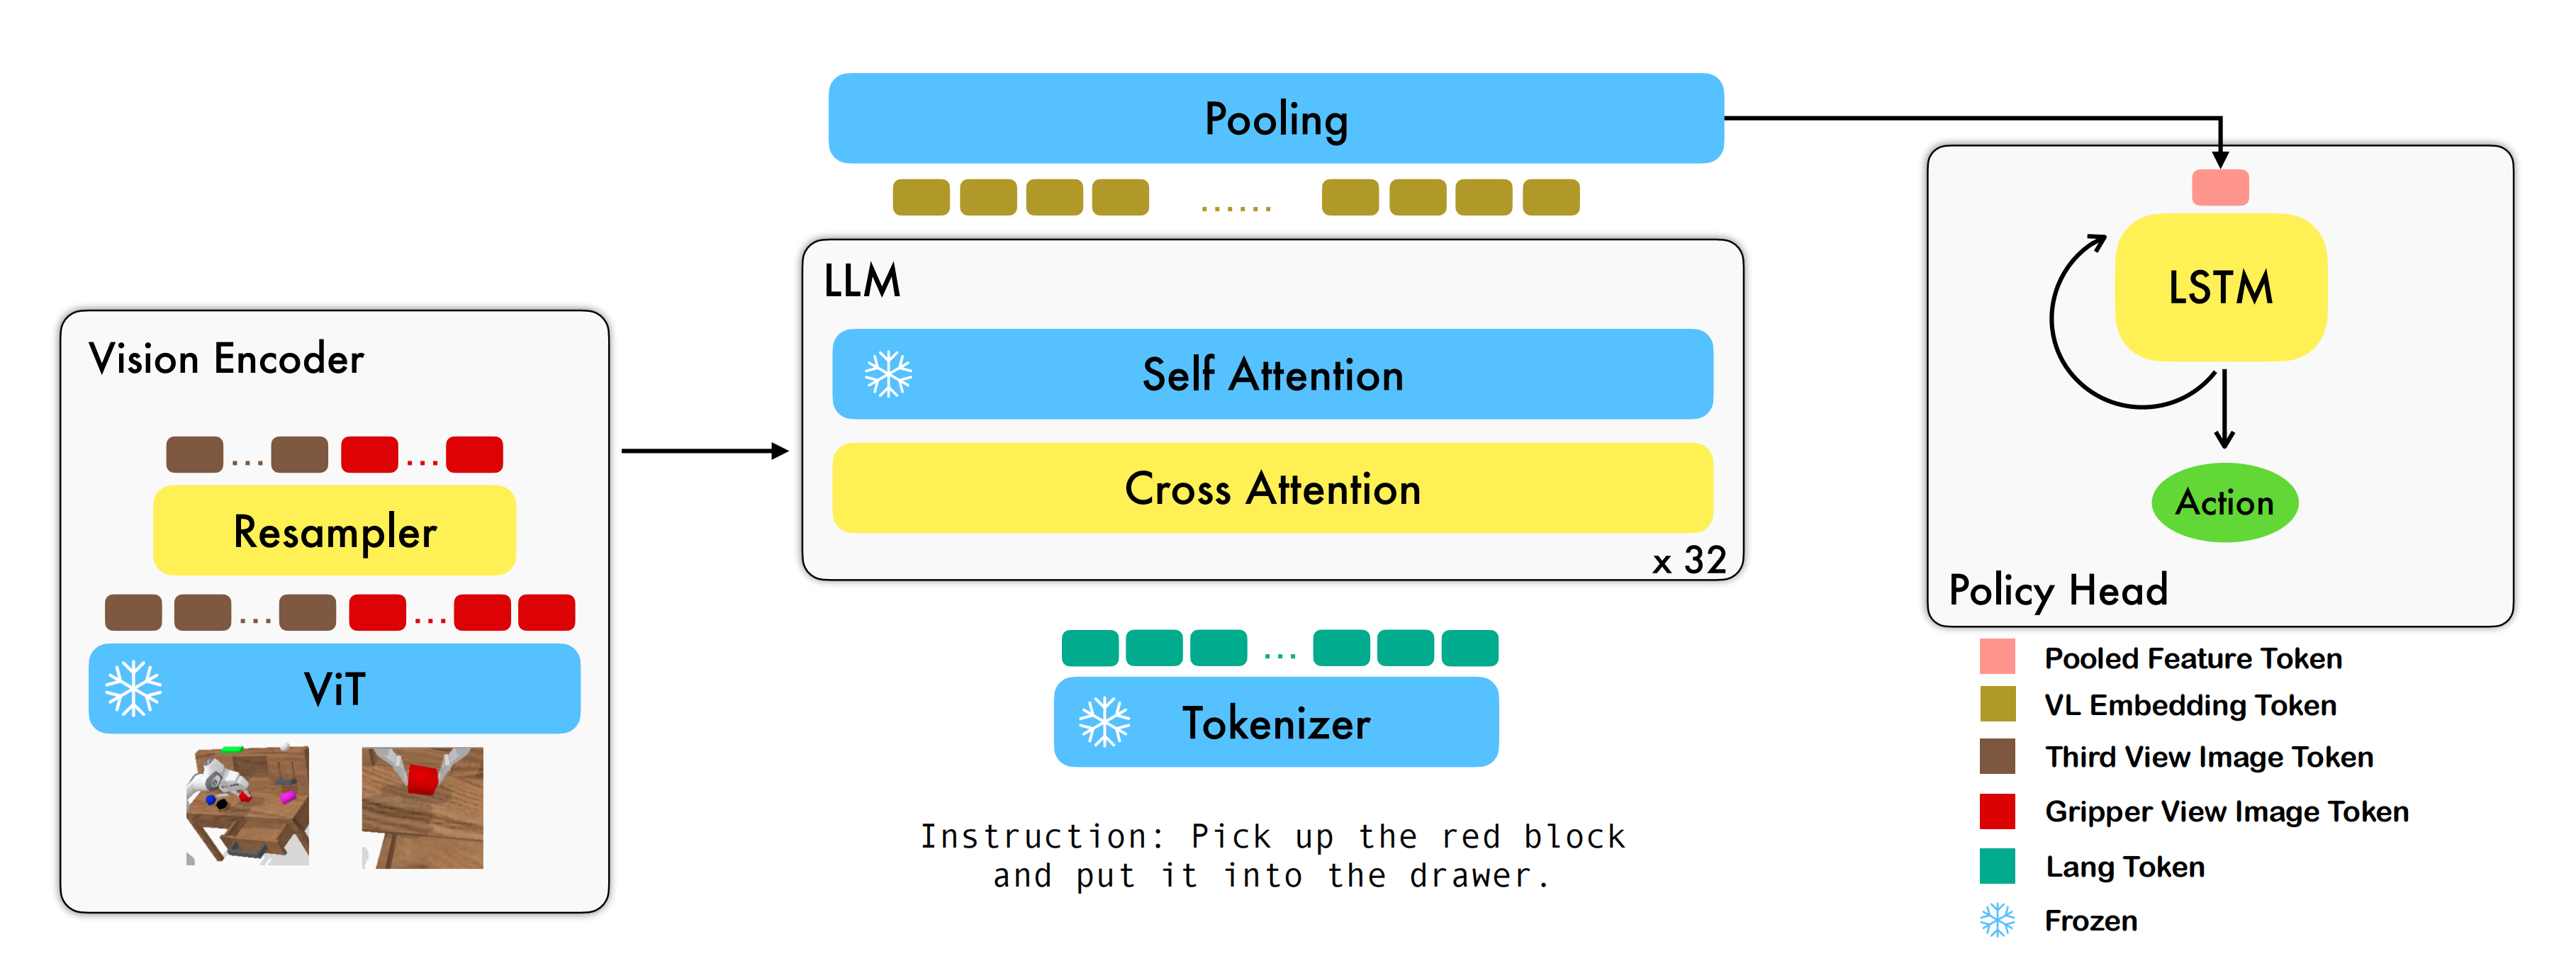
\includegraphics[width=0.9\textwidth]{pic4.png}
\caption{RoboFlamingo}
\end{figure}



\section{计算机视觉}
在实验室看的b站--斯坦福cs231n和鲁鹏老师的课程,记的一些笔记
\subsection{图像分类}
\subsubsection{简单介绍}
数据驱动的图像分类方法:数据集的构建、分类器设计与学习、分类器决策

\begin{figure}[ht]  % 推荐用 [ht] 比 [h] 更稳定
\centering
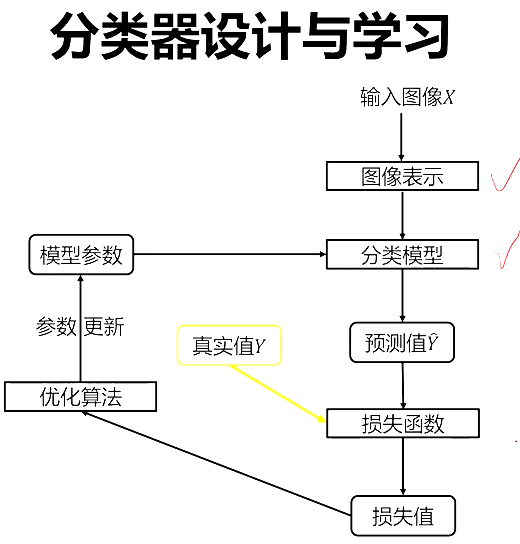
\includegraphics[width=0.4\textwidth]{pic14.png}
\caption{分类器设置与学习}
\end{figure}

过拟合:模型在数据集上表现很好,在未训练数据集决策时表现不好

欠拟合:模型过于简单,怎样拟合都不行

图像表示一般都要向量化

\subsubsection{KNN \(K-Nearest-Neighbors\)}
KNN,全称 K-Nearest Neighbors(K 最近邻算法),是一种常用的监督学习算法,可用于分类和回归问题,尤其在分类中使用较多。
分为两部分,一部分为train,负责训练数据,另一部分负责预测prediction

主要分为两个步骤 :

1.计算所有测试样本与所有训练样本之间的距离

2.在得到这些距离后,对每个测试样本,找到距离它最近的k个训练样本,然后由他们的标签进行“投票”,来预测这个测试样本的标签。
\begin{figure}[ht]  % 推荐用 [ht] 比 [h] 更稳定
\centering
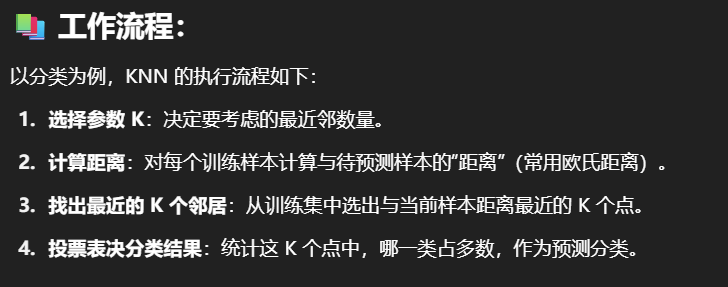
\includegraphics[width=0.6\textwidth]{pic5.png}
\caption{KNN}
\end{figure}
\\L1 \(Manhattan\) distance
\\L2 \(Euclidean\) distance
\\Hyperparameter 超参数:与数据无关,无法通过训练得到的参数,需要在训练前提前设置

当然,KNN也有很明显的缺点,如维数过高时,其需要的训练数据会指数增长,计算时间也会过长

\subsubsection{Linear Classifier}
参数模型中最简单的例子,但通过层级结构(神经网络)或者高维映射(支撑向量机)可以形成强大的非线性功能,通过将图片向量化为参数矩阵,再与特定的Weight进行运算,得到的结果对应class score。
\\$$f_i(x,W_i)=W_i^Tx+b_i$$

x代表输入的d维向量 , $f_i $给出x关于第i类的分数 , where b represents the bias for different classes , W告诉我们x相应像素对class分类的影响。

将所有的$W_i$写为权值矩阵W,可以将上式表示为矩阵形式
\\$$f_i(x,W_i)=W_i^Tx+b_i$$

实际上,对于每类的$W_i$,其维度是10*3072(for CIFAR10),可视化后与该类事物很像,记录的是该类的统计信息,特征越吻合,$W_i$与$x$点乘越大。
\begin{figure}[ht]  % 推荐用 [ht] 比 [h] 更稳定
\centering
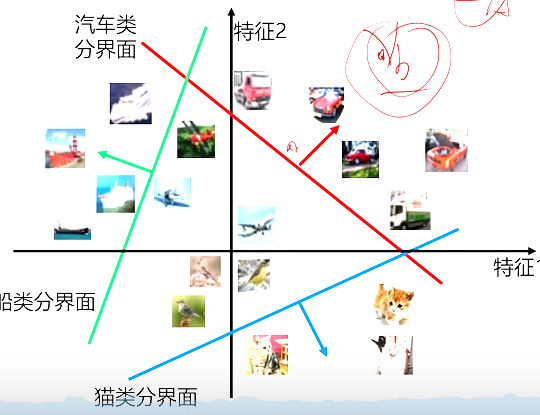
\includegraphics[width=0.6\textwidth]{pic16.png}
\caption{线性分类器}
\end{figure}

由于线性分类器的线性特征,我们在图像上可将其表示为直线,距离直线越近说明与该类特征越接近

但是在面对未训练数据时,线性分类器的准确性就会大打折扣。当面对更多的特征而样本不足时,线性模型往往会过拟合。 相反,当给出更多样本而不是特征,通常线性模型不会过拟合。 不幸的是,线性模型泛化的可靠性是有代价的。 简单地说,线性模型没有考虑到特征之间的交互作用。 对于每个特征,线性模型必须指定正的或负的权重,而忽略其他特征。
\begin{figure}[ht]  % 推荐用 [ht] 比 [h] 更稳定
\centering
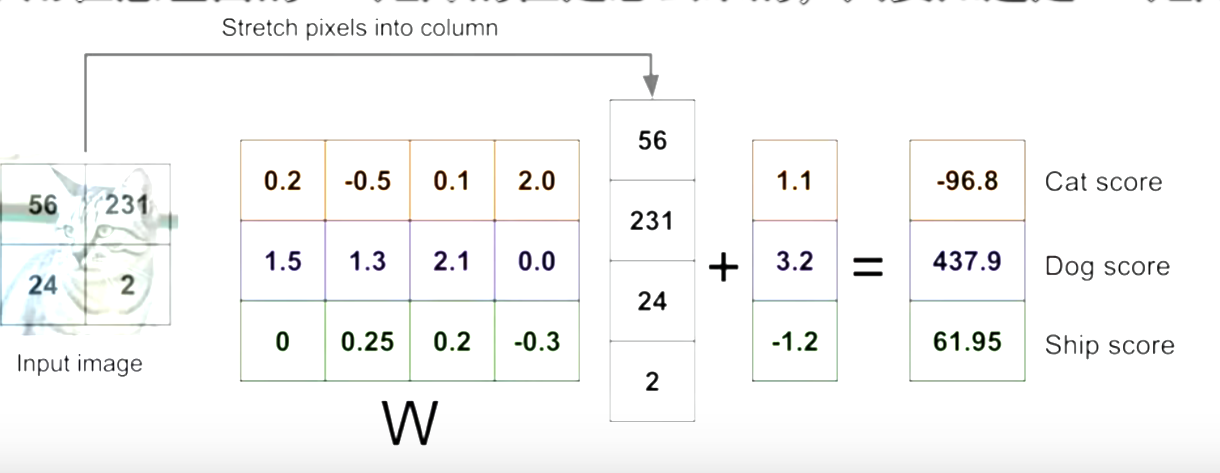
\includegraphics[width=0.7\textwidth]{pic6.png}
\caption{Linear Classifier}
\end{figure}

\subsection{损失函数}
从统计的角度看,我们得到的估计和实际总是有差距的,我们可以得到损失函数,用于度量给定分类器的预测值与真实值的不一致程度:
\\$$ L=\frac{1}{N} \sum_{i}{} L_i(f(x_i,W),y_i)  $$

通过损失函数,我们可以比较W的好坏,并取极值时的W

多类支撑向量机损失
\\$$ L_i=f_j(x_i,W_i,b_j)=\sum_{\substack{j \ne y_i}}^{} \max(0,s_{ij}-s_{yi}+1)       $$

但需要注意的是,假设存在W满足$L=0$,可以看到W并不是唯一的,有些w会使模型太过复杂或阶数过高,我们需要对这些复杂的W加入一个惩罚项,如果要选择这些W就必须客服这些惩罚,所以我们引入R(W),称为正则项,来控制系统的复杂程度。
这样一来,我们的模型就由两部分组成:a data loss and a regularization loss,and there is some hyper-parameter here,$\lambda$,用来平衡这两项
\\$$ L=\frac{1}{N} \sum_{i}^{N} L_i(f(x_i,W),y_i)N+\lambda R(W)  $$

对于L2正则项,$R(W)=\sum_{\substack{k}}\sum_{\substack{l}}W_{k,l}^2$,L2正则项损失对大数值权值经行惩罚,喜欢分散权值,鼓励分类器将所有特征维度都利用起来,而不是强烈的依赖其中少数几维特征

\subsection{Softmax}
让我们进一步探究这些score的含义,同样是对class score的处理,计算每一类别的概率分布,通过指数化来排除干扰,来帮助我们决策,引入\(Softmax\)  \(funnction\):
\\$$P(Y=k|X=x_i)=\frac{e^{s_k}}{\sum_{j}e^{s_j}}$$ 

where 
$$s=f(x_i;W)$$

对于softmax函数,我们的SVM损失函数可以记作
\\$$L_i=-logP(Y=y_i|X=x_i)$$

也就是交叉熵损失,在独热的情况下便退化为上式,本身即
\\$$H(p,q) = -\sum_{i=1}^{c}p(x_i)log(q(x_i)) $$
\begin{figure}[ht]  % 推荐用 [ht] 比 [h] 更稳定
\centering
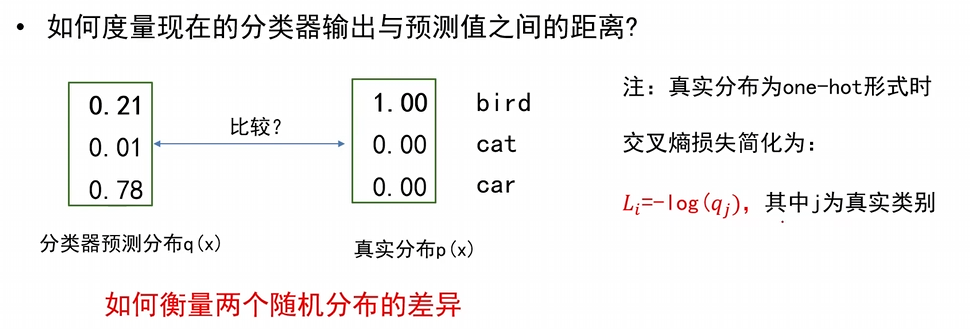
\includegraphics[width=0.7\textwidth]{pic21.png}
\caption{交叉熵损失} 
\end{figure}

相较于之前的比较,Softmax function保留了概率较小的种类,并尽可能向更高概率去优化,而前面的选择方式则是只关心谁更接近,直接抛弃了其他种类,相比之下,Softmax更适合机器学习

\subsection{参数优化}
利用损失函数的输出值作为反馈信号来调整分类器参数,以提升分类器对训练样本的预测性能

\subsubsection{back propagation}
back propagation 反向传播,本质是链式求导法则在神经网络中的应用,通过逐层反向传播误差,逐层计算每个参数对损失函数的影响。特别注意我们的运算是针对向量(矩阵)的,这里有所不同
\begin{figure}[ht]  % 推荐用 [ht] 比 [h] 更稳定
\centering
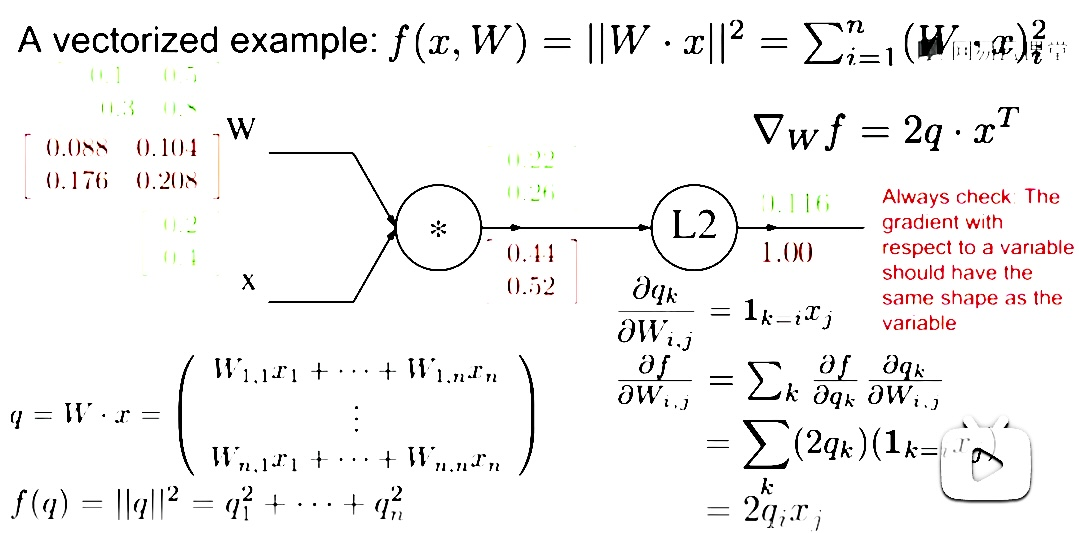
\includegraphics[width=0.7\textwidth]{pic9.jpg}
\caption{对矩阵的运算}
\end{figure}

\subsubsection{梯度下降法}
梯度下降法:而对于$L_i$,我们希望找到他的极值,可以通过求梯度的方式(因为这里W是一个向量,有很多维),确定每次的学习率和步长,每次向负梯度方向增加,可以较快得到最注重的最小值
\\$$\nabla_W L(W)=\frac{1}{N} \sum_{i=1}^{N} \nabla_W L_i(x_i,y_i,W)+\lambda\nabla_W R(W)$$

面对不同的激活函数,尽量选择ReLu或者Leaky ReLU,相对于Sigmode和tanh,其会让梯度流更加顺畅,训练过程收敛更快,具体对比见非线性层一节

注意到,梯度下降法也存在问题,可能“在山壁间震荡,往谷底方向行进缓慢”。于是考虑梯度算法的改进。

\subsubsection{动量法}
利用累加历史梯度信息更新梯度,来加速向山谷移动,或者避免困于局部最小值点,引入动量系数$\mu$,初始化速度为0、学习率为$\epsilon$,则在每次训练中

计算梯度:
$$g\leftarrow \frac{1}{m}\nabla_\theta\sum_{i}L(f(x^{(i)};\theta),y^{(i)}) $$

速度更新:
$$v=v\mu+g$$

更新权值:
$$\theta\leftarrow\theta-\epsilon v$$

\subsubsection{自适应梯度法}
通过减小震荡方向步长,增大平坦方向步长来减小震荡,加速通往谷底。如何判断震荡和平坦?梯度幅度的平方较大的方向就是震荡方向,梯度幅度的平方较小的方向就是平坦方向.初始化累计变量$r=0$,设置$\delta$为小常数,用于被小数除时的数值稳定(通常设为$10^{-5}$),在每次训练时

计算梯度:
$$g\leftarrow \frac{1}{m}\nabla_\theta\sum_{i}L(f(x^{(i)};\theta),y^{(i)}) $$

累计平方梯度:
$$r\leftarrow r+g*g$$

更新权值:
$$\theta \leftarrow \theta -\frac{\epsilon}{\sqrt{r} +\delta}g$$

但注意,该方法也有缺陷,在训练后期r会累积到非常大,导致步长很小,失去调节作用。对此,做出改进:

RMSProp方法:学习率$\epsilon$,衰减速率$\rho$,一般设置为0.999,初始化积累变量$\r=0$

计算梯度:
$$g\leftarrow \frac{1}{m}\nabla_\theta\sum_{i}L(f(x^{(i)};\theta),y^{(i)}) $$

累计平方梯度:
$$r\leftarrow \rho r+(1-\rho)g*g$$

更新权值:
$$\theta \leftarrow \theta -\frac{\epsilon}{\sqrt{r} +\delta}g$$

\subsubsection{Adam}
同时使用动量和自适应梯度思想,学习率$\epsilon$,衰减速率$\rho$,动量系数$\mu$,初始化积累变量$r=0,v=0$,迭代轮次t

计算梯度:
$$g\leftarrow \frac{1}{m}\nabla_\theta\sum_{i}L(f(x^{(i)};\theta),y^{(i)}) $$

累计梯度:
$$v\leftarrow \mu v+(1-\mu)g$$

累计平方梯度:
$$r\leftarrow \rho r+(1-\rho)g*g$$

修正偏差:
$$\widetilde{v}=\frac{v}{1-\mu^t}  ; \widetilde{r}=\frac{r}{1-\rho^t}$$

更新权值:
$$ \theta\leftarrow\theta-\frac{\epsilon}{\sqrt{\widetilde{r}}+\delta}\widetilde{v}$$

注意到,Adam法中加入了修正偏差一项,这是为了缓解算法初期的冷启动问题,在初期$v=0$,而在梯度累计时$v=0+0.1g$,在初期g也很小的情况下会让参数变化很慢,r也存在同样的问题。而在引入修正项后,仅在初期调整梯度积累,防止了冷启动问题,而在后期就与未修正项接近。

\subsubsection{数据预处理}
\begin{figure}[ht]  % 推荐用 [ht] 比 [h] 更稳定
\centering
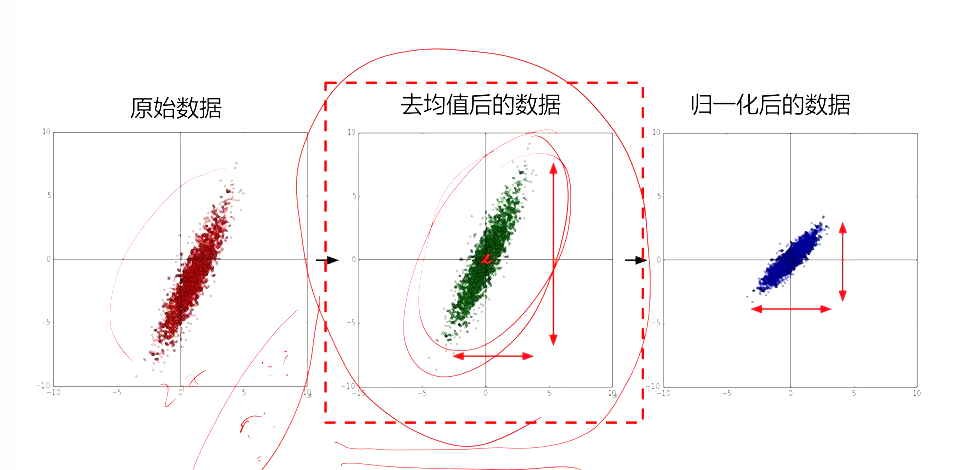
\includegraphics[width=0.7\textwidth]{pic17.png}
\caption{数据预处理1}
\end{figure}
如图10,去均值的数据可以消除样本不同带来的误差(高考分数线每年都不同),归一化则去掉量纲的影响,减去均值除以均值
\begin{figure}[ht]  % 推荐用 [ht] 比 [h] 更稳定
\centering
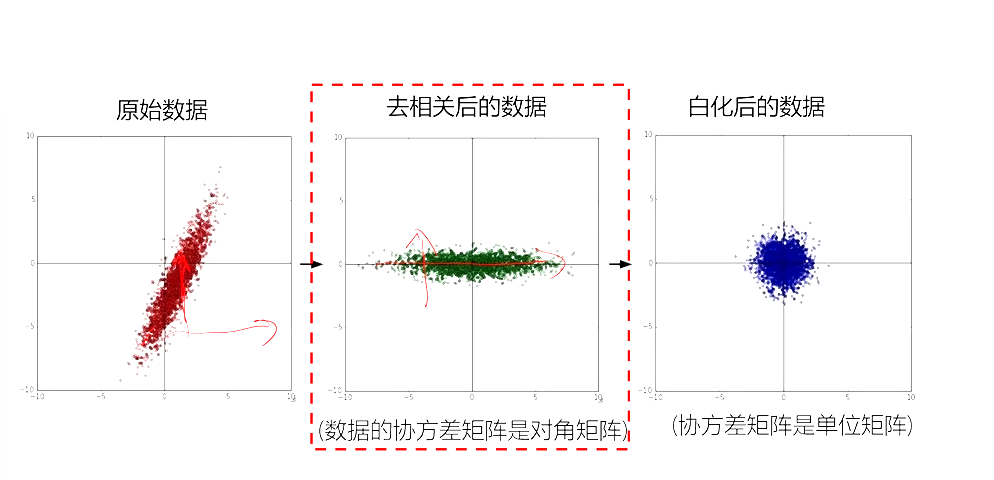
\includegraphics[width=0.7\textwidth]{pic18.png}
\caption{数据预处理2}
\end{figure}
如图11,数据在某一维度上变化非常小,可以去相关,达到降维的效果,再将数据白化

\subsection{全连接神经网络}
受到大脑中神经元的启发,我们发现通过不同函数层的叠加,我们可以得到更加精准高级的得分函数

这种将线性分类器当作神经元组成复杂神经网络的结构也叫做全连接神经网络,也叫多层感知机,其通过级联多个变换来实现输入到输出的映射,多个线性分类器经过非线性操作后级联
\begin{figure}[ht]  % 推荐用 [ht] 比 [h] 更稳定
\centering
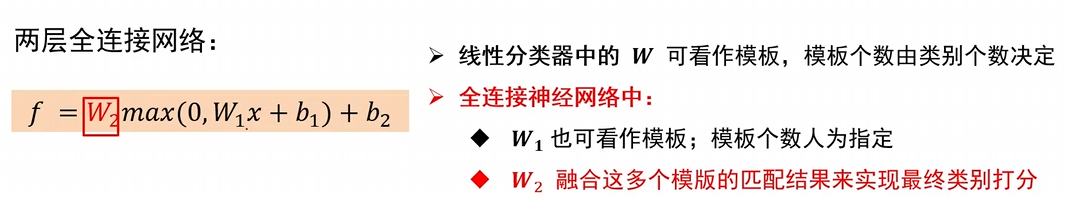
\includegraphics[width=0.8\textwidth]{pic19.png}
\caption{两层全连接网络}
\end{figure}

如果没有非线性函数,多层线性分类器会退化为单层线性分类器,所以必须加上非线性函数,来“激活”这些多层线性分类器,被称为激活函数,常见的激活函数有
\\$$Sigmoid : 1/(1+e^{-x})$$
$$tanh : \frac{e^x-e^{-x}}{e^x+e^{-x}}$$
$$ReLU : max(0,x)$$
$$Leaky ReLU : max(0.1x,x)$$

神经元个数越多,分界面就可以越复杂,在这个集合上的分类能力也就越强。
\begin{figure}[ht]  % 推荐用 [ht] 比 [h] 更稳定
\centering
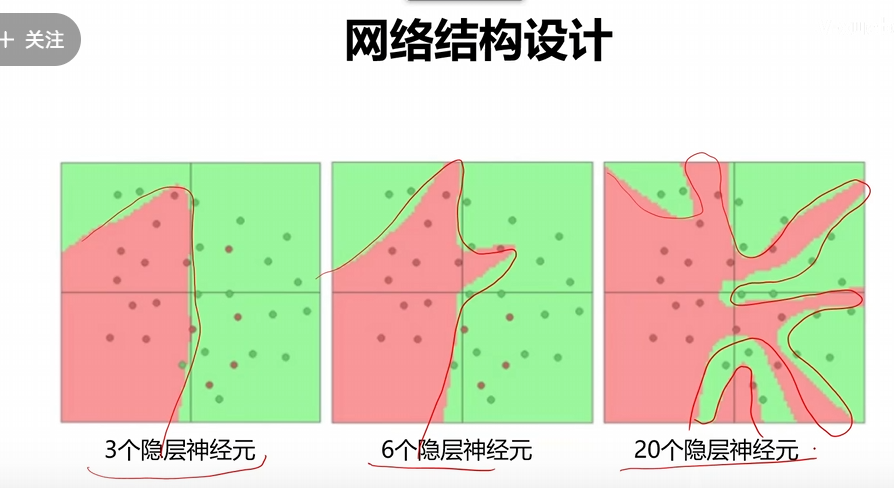
\includegraphics[width=0.6\textwidth]{pic20.png}
\caption{网络结构设计}
\end{figure}

\subsection{训练过程}
\subsubsection{权值初始化}
初始化时让权值不相等,并不能保证网络能够正常的被训练。有效的初始化方法应是使网络各层的激活值和局部梯度的方差在传播过程中尽量保持一致,以保证网络中正向和反向的数据流动,即尽可能让输出零均值一方差。

这里介绍Xavier初始化,权值采样自$\mathcal{N}(0,1/N)$的高斯分布,N为输入的神经元个数

\subsubsection{批归一化}
对输出进行减均值除方差操作;可保证输出零均值一方差。常被放在全连接层与非线性层之间。假设输入为$\mathcal{B} =\{x_1,···,x_m\}$,需要模型自己学习的参数:$\beta ,\gamma$,输出$\{y_1,···,y_2\}$

计算小批量均值:
$$\mu_\mathcal{B}\leftarrow\frac{1}{m}\sum_{m}^{i=1}x_i$$

计算小批量方差:
$$\sigma^2_\mathcal{B}\leftarrow\frac{1}{m}\sum_{m}^{i=1}(x_i-\mu_\mathcal{B})^2$$

归一化:
$$\widehat{x}_i\leftarrow\frac{x_i-\mu_\mathcal{B}}{\sqrt{\sigma^2_\mathcal{B}+\epsilon}}$$ 

平移缩放:
$$y_i\leftarrow\gamma\widehat{x}_i+\beta$$

\subsubsection{过拟合}
过拟合指学习时选择的模型包含参数过多,以至于出现这一模型对已知数据预测得很好,但对位置数据预测的很差的现象。这种情况下模型可能知识记住了训练集数据,而不是学到了数据特征。

机器学习的根本问题是优化和泛化的问题。优化——调节模型以在训练数据上得到最佳性能;泛化——是指训练好的模型在前所未见的数据上的性能好坏

本质上验证集是度量模型泛化能力的工具,可通过观察模型在验证集上的表现来判断其识别能力

应对过拟合的最优方案就是获取更多的训练数据,次优方法还可以调节模型允许存储的信息量或者对模型存储的信息加以约束,该类方法也成为正则化,即$R(W)$项,可尽量控制分界面更为平滑。

\subsubsection{随机失活 dropout}
在训练时让隐层的神经元以一定的概率不被激活,就是将该层的一些输出舍弃(输出值设为0)。通过减小模型参数防止过拟合,同时鼓励权重分散,让每层中的神经元尽可能平均记录特征信息。

dropout还可以看作是模型的集成,每次失活的训练可看作是一个小模型,而在预测时将所有小模型集成到了一起,从而防止过拟合

\subsection{Convolution Neural Networks}
总体与其他神经网络相同,不同的是要训练卷积层,因为卷积层更能保留输入的空间结构

其中可以看到,在归一化x后,我们可以根据模型需要来设置新的数据方差和均值,来调整得到最有利于网络分类的分布

\subsubsection{卷积}
卷积本质上是一种求和的滑动运算,过程可将其视作图像的平移和堆叠,通过卷积核来对图现象进行点乘运算,最简单的
\[
\begin{bmatrix}
0 & 0 & 0\\
0 & 1 & 0\\
0 & 0 & 0
\end{bmatrix}
\]

图像经过上述卷积核后还是自身
\[
\begin{bmatrix}
0 & 0 & 0\\
1 & 0 & 0\\
0 & 0 & 0
\end{bmatrix}
\]

图像经过上述卷积核会进行平移,但自身形状均为发生变化
\[
\begin{bmatrix}
1/9 & 1/9 & 1/9\\
1/9 & 1/9 & 1/9\\
1/9 & 1/9 & 1/9
\end{bmatrix}
\]

经过上述卷积核会让图像整体更加平滑,像素点之间的差别减少,即去噪
\[
\begin{bmatrix}
0 & 0 & 0\\
0 & 1 & 0\\
0 & 0 & 0
\end{bmatrix}
-
\begin{bmatrix}
1/9 & 1/9 & 1/9\\
1/9 & 1/9 & 1/9\\
1/9 & 1/9 & 1/9
\end{bmatrix}
\]

而上述卷积核也叫做平均卷积核,会找到较为突出的像素点,即边缘提取
\[
\begin{bmatrix}
0 & 0 & 0\\
0 & 2 & 0\\
0 & 0 & 0
\end{bmatrix}
-
\begin{bmatrix}
1/9 & 1/9 & 1/9\\
1/9 & 1/9 & 1/9\\
1/9 & 1/9 & 1/9
\end{bmatrix}
\]

上述卷积核则会在原本图像的基础上突出边界,达到锐化的效果

平均卷积核也会带来一些问题,在卷积过后图像会产生一些水平和竖直方向的条状,这一现象叫做振铃。
产生振铃的原因是所有模板的权重都是一样的,我们更希望离像素越近的模板权重越高,而离像素越远的模板权重越低,
所以来进一步改进我们的卷积核,考虑一种最常见的符合要求的卷积核——高斯卷积核
\subsubsection{Convolution Layer}
一般的神经网络会将转化为很小的矩阵,通过矩阵的值来判断类别,如下图
\begin{figure}[ht]  % 推荐用 [ht] 比 [h] 更稳定
\centering
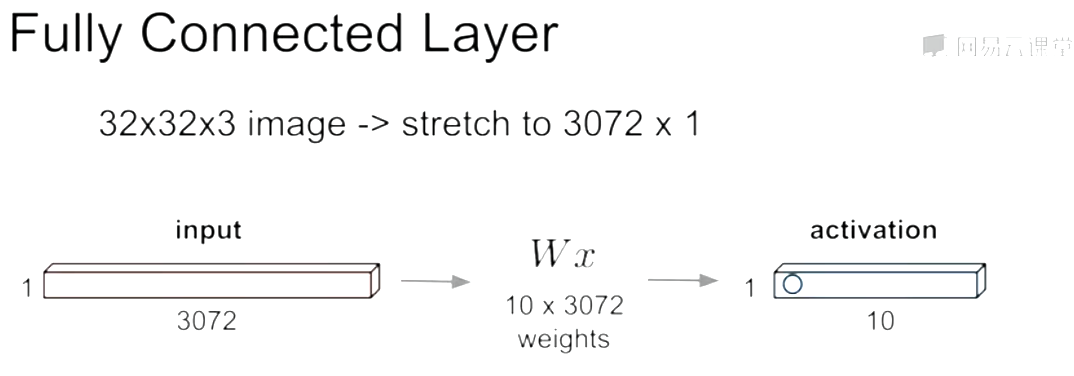
\includegraphics[width=0.7\textwidth]{pic10.png}
\caption{3-layer neural net}
\end{figure}

而CNN则通过多个较小的向量filter(卷积核),来分区滑动对图片进行点乘,尽可能保存图片原本的规模
 \begin{figure}[ht]  % 推荐用 [ht] 比 [h] 更稳定
\centering
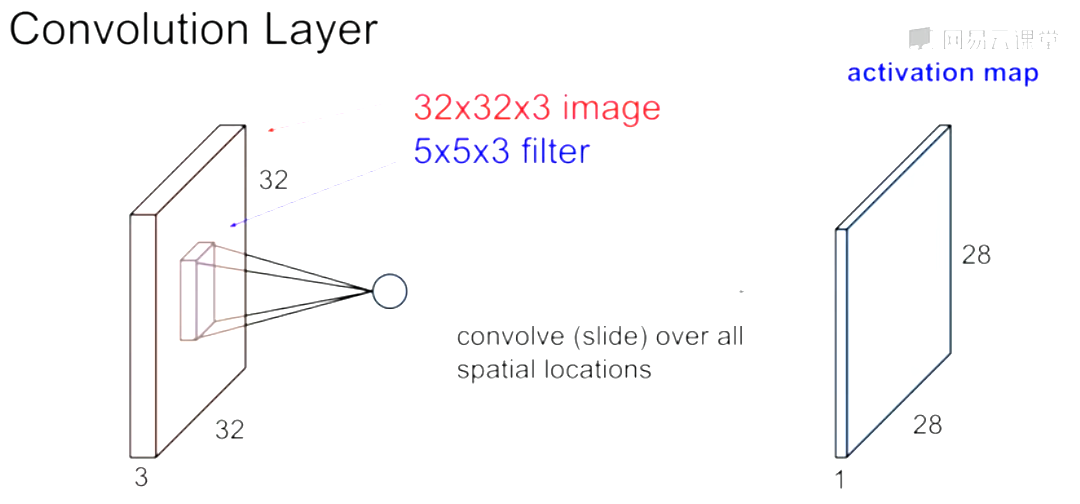
\includegraphics[width=0.7\textwidth]{pic11.png}
\caption{3-layer neural net}
\end{figure}
但是在每层卷积过后,我们图片的规模总会减小(这与我们卷积核的宽度有关),我们知道正常的模型总要经过多层卷积,
但是如果直接卷积就会导致我们的图片shrink extremely,带来信息的损失, 所以我们采取在图片向量周围补0(pad)的措施。
\begin{figure}[ht]  % 推荐用 [ht] 比 [h] 更稳定
\centering
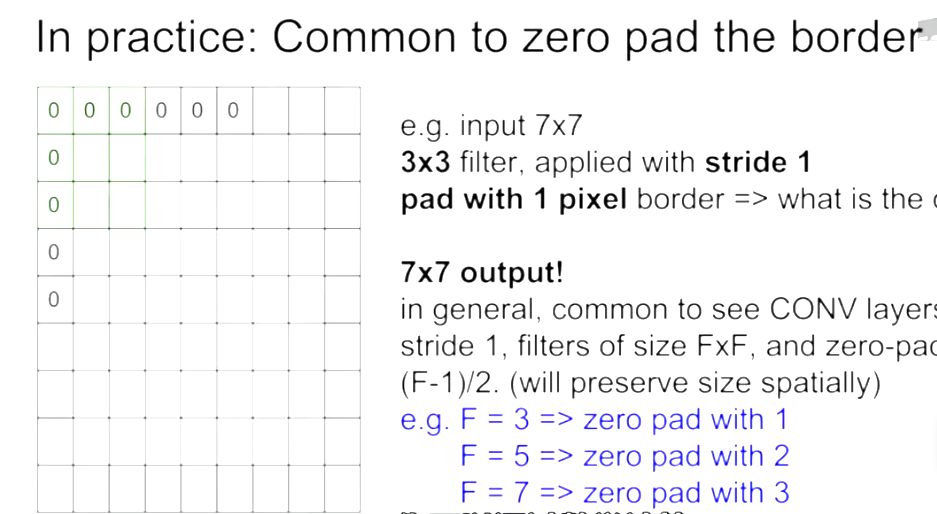
\includegraphics[width=0.7\textwidth]{pic12.png}
\caption{3-layer neural net}
\end{figure}

还应注意,卷积核是有深度的,其深度默认和输入深度一一致。
\\例题:input volume:32*32*3 and 10 5*5 filters with stride 1,pad 2
\\1.The output volume size?
\\$$(32-5+2\times2)//1+1\times=32$$

so it's 32*32*10
\\2.Number of parameters in this layer?
\\$$(5\times5\times3+1)\times10$$

还要加上偏置项b的1

\subsubsection{Pooling Layer}
池化(Pooling)操作是CNN中常用的一种下采样(downsampling)方法,其核心目的是降低特征图的空间维度(宽度和高度),从而:
降低计算量和参数数量、增强特征的平移不变性(translation invariance)、抑制过拟合

其只对参数进行采样,并不影响深度,常见的池化还有最大池化、平均池化

\subsubsection{Rectified Linear Unit}
非线性层,线性整流函数是深度学习中最常用的激活函数之一,主要用于引入非线性,使神经网络能拟合更复杂的函数,通常在卷积层或全连接层之后使用。对于一个输入x,ReLU 函数定义为:
\\$$ReLU(x)=max(0,x)$$

为什么使用 ReLU?

1.非线性但计算简单(不像 sigmoid 那样涉及指数运算)

2.缓解梯度消失问题(sigmoid/tanh 在远离0处导数趋近于0,而 ReLU 在正区间导数为1)

3.稀疏激活(Sparsity):负值会被直接截断为0,让一部分神经元“沉默”,有助于简化表示与泛化能力。
\begin{figure}[ht]  % 推荐用 [ht] 比 [h] 更稳定
\centering
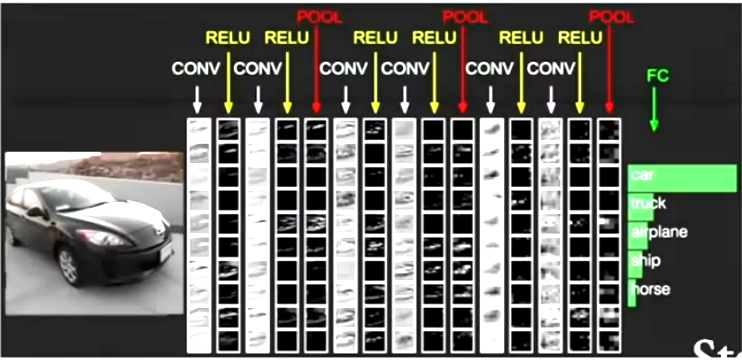
\includegraphics[width=0.7\textwidth]{pic13.png}
\caption{the CNN}
\end{figure}

\subsection{CPU \& GPU}
CPU,Central Processing Unit,小芯片

GPU,Graphics Processinng Unit,大块头,被称作图形卡或者图形处理单元,最初用于渲染计算机图形(尤其在游戏领域),
核多,每个核相较于CPU运行速度非常缓慢,且可执行的操作没有CPU多,无法单独执行某一项任务,需要共同执行同一项任务。
CPU做通讯处理比较出色,GPU更擅长并行运算某些算法,一项GPU非常擅长的运算就是矩阵乘法,在计算卷积神经网络时,
GPU可以将矩阵计算快速分配到多个核中进行运算,这也是为什么GPU比CPU更适用于CNN


\section*{参考文献}
\bibliographystyle{plainnat}
\bibliography{ref}

\end{document}



%\lstinputlisting[
%    style=verilog-style,
    %caption={\bfseries top\_module.v},
%    label={lst:topmodule} 
%]{top_module.v}